\documentclass{article}
\usepackage{graphicx} % Required for inserting images
\usepackage{amsmath, amsfonts, amssymb}
\usepackage[dvipsnames]{xcolor}
\usepackage{xcolor}
\usepackage{bbold}
\usepackage{float}
\usepackage{subcaption}
\usepackage{tikz}
\usepackage{logicpuzzle}
\usepackage{hyperref}
\usepackage{listings}
\usepackage{mdframed}
\usepackage[numbered,framed]{matlab-prettifier}
\lstset{
   style              = Matlab-editor,
   basicstyle         = \mlttfamily ,
   escapechar         = ",
   mlshowsectionrules = true,
}


% ========= Bibliography =========
% These lines load the `biblatex' package
% and read in the list of references from
% References.bib - take a look.
%
% To generate References.bib, I recommend https://www.mybib.com/
% rather than trying to write the .bib file yourself.
%
\usepackage{csquotes, biblatex}
\addbibresource{References.bib}
% ================================


\newtheorem{prop}{Proposition} % This defines a theorem-like environment. See https://www.overleaf.com/learn/latex/theorems_and_proofs
\newtheorem{lem}[prop]{Lemma}
\newtheorem{thm}[prop]{Theorem}
\newtheorem{cor}[prop]{Corollary}
\newtheorem{defn}[prop]{Definition}

\tikzset{thck/.style={black,line width=2pt},thn/.style={black,line width=0.5pt}}
\newcommand{\sudoku}[1]{%
    \begin{tikzpicture}
        \draw[thn] (0,0) grid (9,9);
        \draw[thck,line cap=rect] (0,0) grid[step=3] (9,9);
        
        \foreach \n [count=\i from 0] in {#1}
            {
            \pgfmathtruncatemacro{\x}{Mod(\i,9)}
            \pgfmathtruncatemacro{\y}{\i/9)}
            \node at (\x+0.5,9-\y-0.5) {\n};
            }
    \end{tikzpicture}
    }

\title{Quadratic Unconstrained Binary Optimization}
\author{Sam Muir }
\date{June 2024}

\begin{document}

\maketitle

\section{Introduction}

The Quadratic Unconstrained Binary Optimization (QUBO) problem is an optimization problem which consists of finding the binary vector that minimizes a quadratic function.
The QUBO model encompasses many important combinatorial optimization problems which have applications in computer science, operations research and physics.\\
QUBO problems are also at the forefront of quantum computing since they are particularly well-suited to being solved using quantum annealing.\\

\noindent In this project we begin by covering how QUBO models can be constructed. Then we will explore QUBO formulations of some well known combinatorial problems. We then apply these insights to the graph matching problem and the related quadratic assignment problem. Finally, we discuss the feasibility of using quantum annealers to solve QUBO problems. \\

\noindent This project will follow 'Continuous optimization methods for the graph isomorphism problem' by Stefan Klus and Patrick Gelß. This report will also contain MATLAB code showing QUBO implementations of each problem. This code can also be found at \href{https://github.com/muirsam/QUBO/}{https://github.com/muirsam/QUBO/}

\section{What are QUBO problems?}
\begin{defn}
A QUBO problem is an optimisation problem of form
\begin{align*}
    \min_{\mathbf{x} \in B(n)} \: f(\mathbf{x}) = \mathbf{x}^T Q \mathbf{x} + d,
\end{align*}
where \(B(n)\) is the set of vectors with \(n\) binary entries, \(Q \in \mathbb{R}^{n \times n}\) and \(d \in \mathbb{R}\).
\end{defn}

\noindent Note that since \(d\) is a constant, we can omit it without changing the optimal solution of the function.\\

\noindent At first glance this definition seems quite limited. But using a few tricks we can convert many problems to this form.

\subsubsection{Simple Example}
\noindent Suppose we are given a set of four numbers \(\alpha = \{\alpha_1,\alpha_2, \dots \alpha_4\}\) and we need to find the two-element subset of \(\alpha\) with the largest sum. We can convert this into a QUBO problem as follows. \\

\noindent First define the binary decision vector \(\mathbf{x} = \begin{pmatrix}
	x_1 & x_2 & x_3 & x_4
	\end{pmatrix}^T\). 
Then the sum function can be written as \(\sum_{i=1}^4 \alpha_i x_i\). But since \(x_i\) is binary, \(x_i = x_i^2\) and so we can express the sum function as
\begin{align*}
\sum_{i=1}^4 \alpha_i x_i = \sum_{i=1}^4 \alpha_i x_i^2 = \mathbf{x}^T\begin{pmatrix}
	\alpha_1 & 0 & 0 & 0 \\
	0 & \alpha_2 & 0 & 0 \\
	0 & 0 & \alpha_3 & 0 \\ 
	0 & 0 & 0 & \alpha_4
\end{pmatrix}\mathbf{x}.
\end{align*} 
\noindent Maximising this function will give the subset with the largest sum. But we want the largest two-element subset so we need to add a penalty term to guarantee that the solution is a two-element subset. \\
By writing the two-element constraint as \(\sum_{i=1}^n x_i = 2\), we can construct the penalty 
\begin{align*}
    \bigg(\sum_{i=1}^4 x_i - 2\bigg)^2 = \sum_{i=1}^4 x_i\sum_{j=1}^4 x_j - 4\sum_{i=1}^4 x_i + 4
\end{align*}
\noindent which is 0 for two-element subsets and positive otherwise. Then since \(x_i = x_i^2\) this penalty is a quadratic form plus a constant
\begin{align*}
	\bigg(\sum_{i=1}^4 x_i - 2\bigg)^2 &= \sum_{i=1}^4\sum_{j=1}^4 x_ix_j - 4\sum_{i=1}^4 x_i^2 + 4 \\
	&= \mathbf{x}^T \begin{pmatrix}
		1 & 1 & 1 & 1 \\
		1 & 1 & 1 & 1 \\
		1 & 1 & 1 & 1 \\
		1 & 1 & 1 & 1
	\end{pmatrix}\mathbf{x} +\mathbf{x}^T \begin{pmatrix}
		-4 & 0 & 0 & 0 \\
		0 & -4 & 0 & 0 \\
		0 & 0 & -4 & 0 \\
		0 & 0 & 0 & -4 
	\end{pmatrix}\mathbf{x} + 4 \\
	&= \mathbf{x}^T \begin{pmatrix}
		-3 & 1 & 1 & 1 \\
		1 & -3 & 1 & 1 \\
		1 & 1 & -3 & 1 \\
		1 & 1 & 1 & -3
	\end{pmatrix} \mathbf{x} + 4.
\end{align*}
Since the sum of \(\alpha\) is bounded above by \(\lambda = \sum_{i=1}^4 |\alpha_i|\) and the penalty is a positive integer we have
\begin{align*}
    \lambda \bigg(\sum_{i=1}^4 x_i - 2\bigg)^2 \geq \sum_{i=1}^4 \alpha_i x_i 
\end{align*}
for subsets which do not have exactly two elements. Then we can construct the function
\begin{align*}
    \sum_{i=1}^4 \alpha_i x_i - 2\lambda \bigg(\sum_{i=1}^4 x_i - 2\bigg)^2
\end{align*}
which is equal to the sum function for a two-element subset and less than or equal to \(-\lambda\) otherwise. But \(-\lambda\) is also a lower bound for the sum and therefore the optimal value of this function will be the two-element subset with the largest sum.

\noindent So the function we want to maximise is
\begin{align*}
    &\sum_{i=1}^4 \alpha_i x_i - 2\lambda \bigg(\sum_{i=1}^4 x_i - 2\bigg)^2 \\ =& \: \mathbf{x}^T\begin{pmatrix}
		\alpha_1 & 0 & 0 & 0 \\
		0 & \alpha_2 & 0 & 0 \\
		0 & 0 & \alpha_3 & 0 \\ 
		0 & 0 & 0 & \alpha_4
	\end{pmatrix} - 2 \lambda \mathbf{x}^T \begin{pmatrix}
	-3 & 1 & 1 & 1 \\
	1 & -3 & 1 & 1 \\
	1 & 1 & -3 & 1 \\
	1 & 1 & 1 & -3
	\end{pmatrix} \mathbf{x} - 8\lambda.
\end{align*}

\noindent Now we can now write the problem as
\begin{align*}
	\max_{\mathbf{x} \in B(n)} \: \mathbf{x}^T \begin{pmatrix}
        \alpha_1 + 6\lambda & -2\lambda & -2\lambda & -2\lambda \\
        -2\lambda  & \alpha_2 + 6\lambda  & -2\lambda & -2\lambda\\
        -2\lambda & -2\lambda & \alpha_3 + 6\lambda & -2\lambda \\
        -2\lambda & -2\lambda & -2\lambda & \alpha_4 + 6\lambda
	\end{pmatrix} \mathbf{x} - 8\lambda.
\end{align*}
Then we can negate this and omit the constant term to get
\begin{align*}
    \min_{\mathbf{x} \in B(n)} \: \mathbf{x}^T \begin{pmatrix}
        -\alpha_1 - 6\lambda & 2\lambda & 2\lambda & 2\lambda \\
        2\lambda  & -\alpha_2 - 6\lambda & 2\lambda & 2\lambda\\
        2\lambda & 2\lambda & -\alpha_3 - 6\lambda & 2\lambda \\
        2\lambda & 2\lambda & 2\lambda & -\alpha_4 - 6\lambda
	\end{pmatrix} \mathbf{x}
\end{align*}
where \(\lambda = \sum_{i=1}^4 |\alpha_i|\). This is the QUBO formulation of the problem.\\

\noindent We can solve this QUBO in MATLAB as follows
\begin{lstlisting}[language=MATLAB]
a = [a_1, a_2, a_3, a_4];
weight = sum(abs(a));
Q = diag(-a - 8*weight) + 2*weight*ones(4);

solve(qubo(Q))
\end{lstlisting} 

\noindent In this example we were able to find a theoretical penalty weight \(\lambda\) which ensured the solutions were two-element subsets. For most sets \(\alpha\) we could have used a smaller weight and obtained the same solution.\\
Since it is not always practical to derive the optimal weight and larger weights increase the runtime of most QUBO solvers, it is common practise to estimate the weights and check the solution for feasibility instead. \\

\noindent For more examples and a list of penalties corresponding to more complicated constraints, see \cite[p.~10]{tutorialQUBO}. This tutorial improved my understanding of QUBO problems immensely.\\

\subsection{Maximal Independent Set problem}

\noindent The maximal independent set of a graph is the largest subset of the vertex set such that no two vertices share an edge.

\begin{figure}[H]
    \centering
    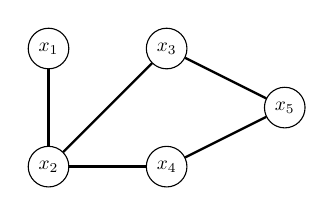
\begin{tikzpicture}
        \node[shape=circle,draw=black, scale=0.7] (A) at (0, 0) {\(x_1\)};
        \node[shape=circle,draw=black, scale=0.7] (B) at (0, -1.5) {\(x_2\)};
        \node[shape=circle,draw=black, scale=0.7] (C) at (1.5, 0) {\(x_3\)};
        \node[shape=circle,draw=black, scale=0.7] (D) at (1.5, -1.5) {\(x_4\)};
        \node[shape=circle,draw=black, scale=0.7] (E) at (3, -0.75) {\(x_5\)};
    
        \path [line width=0.3mm] (A) edge node[left] {} (B);
        
        \path [line width=0.3mm] (B) edge node[left] {} (C);
        \path [line width=0.3mm] (B) edge node[left] {} (D);

        \path [line width=0.3mm] (E) edge node[left] {} (C);
        \path [line width=0.3mm] (E) edge node[left] {} (D);
    \end{tikzpicture}
    \caption{This graph has maximal independent set \{\(x_1, x_3, x_4\)\}.}
\end{figure}

\noindent The maximal independent set problem is identifying the maximal independent set. We can create a QUBO formulation of this problem as follows. \\

\noindent Suppose the vertices of the graph are labelled \(x_1, \dots,  x_n\). For each edge connecting vertices \(x_i\) and \(x_j\), we add the constraint \(x_i + x_j \leq 1\). \\ This constraint corresponds to the penalty \(2x_ix_j - x_i - x_j\) which is \(0\) when both vertices are included and \(-1\) otherwise. Since \(x_a = x_a^2\) this penalty becomes
\begin{align*}
    2x_ix_j - x_i - x_j &= 2x_ix_j - x_i^2 - x_j^2 \\
    &= \begin{pmatrix}
        x_i & x_j
    \end{pmatrix} \begin{pmatrix}
        -1 & 1 \\
         1 & -1 
    \end{pmatrix}
    \begin{pmatrix}
        x_i \\
        x_j
    \end{pmatrix}.
\end{align*}
\noindent This penalty can then be expressed as \(\mathbf{x}^T P_{E_{ij}}\mathbf{x}\) where \(P_{E_{ij}}\) is the matrix of zeros except at the intersections of rows \(i\) and \(j\) and columns \(i\) and \(j\). The entries at the intersections on the main diagonal are \(-1\) and the others are \(1\).\\

\noindent Since the penalties are \(-1\) when one vertex is not excluded and 0 otherwise, the maximal independent set will be the subset which minimises the sum of these penalties. So the maximal independent set corresponds to the solution of
\begin{align*}
    \min_{\mathbf{x} \in B(n)} \: \mathbf{x}^T Q \mathbf{x}.
\end{align*}
where \(Q = \sum_{E_{ij} \in E} P_{E_{ij}}\) and \(E\) is the set of edges of the graph.\\

\noindent Letting \(A\) be the adjacency matrix of the graph we can solve this in MATLAB as follows
\begin{lstlisting}[language=MATLAB]
Q = zeros(n);
for i=1:n
    for j=1:n
        if A(i,j) == 1
            Q(i,i) = Q(i,i) - weight;
            Q(i,j) = Q(i,j) + weight;
        end
    end
end

solve(qubo(Q))
\end{lstlisting}

\subsection{Linear Assignment problem}

The linear assignment problem can be stated as:

Suppose we have \(n\) machines and \(n\) tasks which must be completed. We can assign any machine to do any task, but each task-machine pair has an associated cost. We want to allocate one machine to each task such that the sum of the costs is minimised. \\

\noindent If we let \(A\) be the matrix of machine-task costs then the problem can be expressed as: 
\begin{align*}
    \min_{P \in \mathcal{P}(n)} \: g(P) = \text{tr}(PA)
\end{align*}
where \(\mathcal{P}(n)\) is the set of all \(n \times n\) permutation matrices. \\

\noindent We model this problem as a QUBO as follows. First, let 
\begin{align*}
    A = \begin{pmatrix}
    a_{11} & \hdots & a_{1n} \\
    \vdots & \ddots & \vdots \\
    a_{n1} & \hdots & a_{nn}
\end{pmatrix}, \quad P = \begin{pmatrix}
    x_{1} & x_2 & \hdots & x_{n} \\
    x_{n + 1} & x_{n + 2} & \hdots & x_{2n} \\
    \vdots & \vdots & \ddots & \vdots \\
    x_{n(n-1)+1} & x_{n(n-1)+2} & \hdots & x_{n^2}
\end{pmatrix}
\end{align*}

\noindent Then the function to be minimized is,
\begin{align*}
    \text{tr} (PA) &= \begin{pmatrix}
        x_1 \\
        \vdots \\
        x_n
    \end{pmatrix} \cdot \begin{pmatrix}
        a_{11}\\
        \vdots \\
        a_{n1}
    \end{pmatrix} + \begin{pmatrix}
        x_{n+1} \\
        \vdots \\
        x_{2n}
    \end{pmatrix} \cdot \begin{pmatrix}
        a_{12}\\
        \vdots \\
        a_{n2}
    \end{pmatrix} + \hdots + \begin{pmatrix}
        x_{n(n-1) + 1} \\
        \vdots \\
        x_{n^2}
    \end{pmatrix} \cdot \begin{pmatrix}
        a_{1n}\\
        \vdots \\
        a_{nn}
    \end{pmatrix} \\
    &= \sum_{i=1}^{n} \begin{pmatrix}
        x_{n(i-1) + 1} \\
        \vdots \\
        x_{ni}
    \end{pmatrix} \cdot \begin{pmatrix}
        a_{1i} \\
        \vdots \\
        a_{ni}
    \end{pmatrix} \\
    &= \sum_{i=1}^{n} \sum_{j=1}^{n} a_{ji}x_{n(i-1)+j}
\end{align*}
But \(x_i\) is binary so \(x_i = x_i^2\), and 
\begin{align*}
    \text{tr}(PA) &= \sum_{i=1}^{n} \sum_{j=1}^{n} a_{ji}x_{n(i-1)+j} \\
    &= \mathbf{x}^T \text{diag}(\text{vec}(A))\mathbf{x}
\end{align*}
where vec\((A) = \begin{pmatrix}
    A_1 \\
    \vdots \\
    A_n
\end{pmatrix}\) and \(A_1, \dots A_n\) are the columns of \(A\).\\

\noindent So we can write the problem as 
\begin{align} \label{Ex:LinAss 1}
    \min g(\mathbf{x}) = \mathbf{x}^T \text{diag}(\text{vec}(A)) \mathbf{x}
\end{align}
where \(\mathbf{x} = \text{vec}(P^T)\) and \(P\) is a permutation matrix.\\

\noindent Now we need a penalty function which forces \(P\) to be a permutation matrix. To accomplish this we use the equation \(C\mathbf{x} = d\) given in \cite[p.~8]{klus2023continuous} where 
\begin{align}\label{mat:CD}
    C = \begin{pmatrix}
        \mathbb{1}_n^T & & \\
         & \ddots & \\ 
         & & \mathbb{1}_n^T \\
         e_1^T & \hdots & e_1^T \\
         \vdots & \ddots & \vdots \\
         e_n^T & \hdots & e_n^T
    \end{pmatrix} \in \mathbb{R}^{2n \times n^2}, \quad d = \mathbb{1}_{2n}
\end{align}
with \(\mathbb{1}_n\) is the vector of \(n\) ones and \(e_i\) is the \(i\)th standard basis vector (with \(n\) entries). \\

\noindent This equation is 0 if and only if \(P\) is doubly stochastic. But if \(P\) is doubly stochastic it is also a permutation matrix since each entry is binary. So this constraint forces \(P\) to be a permutation matrix.\\

\noindent We can transform the constraint \(C\mathbf{x} = d\) into the penalty \((C\mathbf{x} - d) \cdot (C\mathbf{x} - d)\). Adding this to (\ref{Ex:LinAss 1}) will favour solutions which are  permutation matrices.
Expanding this penalty we get,
\begin{align*}
    (C\mathbf{x} - d) \cdot (C\mathbf{x} - d) &= C\mathbf{x} \cdot C\mathbf{x} - 2d\cdot C\mathbf{x} + d \cdot d \\
    &= \mathbf{x}^T C^T C \mathbf{x} -2\mathbf{x}^T C^T d + d^Td
\end{align*}

\noindent Then since \(\mathbf{x}\) is binary \(x_i = x_i^2\) the linear term \(-2\mathbf{x}^T C^T d\) can be expressed as the quadratic term \(-2\mathbf{x}^T\text{diag}(C^Td)\mathbf{x}\). So the penalty term becomes
\begin{align}
    &\mathbf{x}^T C^T C \mathbf{x} -2\mathbf{x}^T\text{diag}(C^Td)\mathbf{x} + d^Td \nonumber \\
    = \: &\mathbf{x}^T(C^T C -2\text{diag}(C^Td))\mathbf{x} + d^Td. \label{penalty:CX}
\end{align}
And so we can rewrite problem (\ref{Ex:LinAss 1}) as 
\begin{align*}
    \min g(\mathbf{x}) = \mathbf{x}^T (\text{diag}(\text{vec}(A)) + \lambda C^T C - 2\lambda\text{diag}(C^T d))\mathbf{x} + \lambda d^Td
\end{align*}
where \(\lambda\) is the penalty weight. Then we can drop the constant to get
\begin{align*}
    \min g(\mathbf{x}) = \mathbf{x}^T Q \mathbf{x}
\end{align*}
where \(Q = \text{diag}(\text{vec}(A) - 2\lambda C^Td) + \lambda C^T C\).\\

\noindent This can be solved with the code:
\begin{lstlisting}[language=MATLAB]
Ct = transpose(C)
v = reshape(A, 1, [])
Q = diag(v - weight*2*Ct*d) + weight*Ct*C

x = solve(qubo(Q));
P = transpose(reshape(x.BestX, n, []))
\end{lstlisting}

\subsubsection{Example: Linear Assignment problem}

Consider the cost matrix \begin{align*}
    A = \begin{pmatrix}
        7 & 9 & 1\\
        4 & 2 & 6\\
        7 & 8 & 7
    \end{pmatrix},
\end{align*}
where each column corresponds to a task and each row corresponds to the machine costs.

\noindent Using \(A\) and setting \(\lambda = 10\) we obtain the matrix
\begin{align*}
    Q = \begin{pmatrix}
        -13 & 10 & 10 & 10 & 0 & 0 & 10 & 0 & 0 \\
        10 & -16 & 10 & 0 & 10 & 0 & 0 & 10 & 0 \\
        10 & 10 & -13 & 0 & 0 & 10 & 0 & 0 & 10 \\
        10 & 0 & 0 & -11 & 10 & 10 & 10 & 0 & 0 \\
        0 & 10 & 0 & 10 & -18 & 10 & 0 & 10 & 0 \\
        0 & 0 & 10 & 10 & 10 & -12 & 0 & 0 & 10 \\
        10 & 0 & 0 & 10 & 0 & 0 & -19 & 10 & 10 \\
        0 & 10 & 0 & 0 & 10 & 0 & 10 & -14 & 10 \\
        0 & 0 & 10 & 0 & 0 & 10 & 10 & 10 & -13
    \end{pmatrix}.
\end{align*}
Solving this gives \(X = \begin{pmatrix}
    0 & 0 & 1 & 0 & 1 & 0 & 1 & 0 & 0
\end{pmatrix}^T\)
and so we have \begin{align*}
    P = \begin{pmatrix}
        0 & 0 & 1 \\
        0 & 1 & 0 \\
        1 & 0 & 0
    \end{pmatrix}, \quad PA = \begin{pmatrix}
        7 & 8 & 7 \\
        4 & 2 & 6 \\
        7 & 9 & 1
    \end{pmatrix}
\end{align*}
which tells us that the minimum cost is \(\text{tr}(PA) = 10\).
\subsection{Sudoku}

In the game of Sudoku we are given a partially filled \(9 \times 9\) grid (81 squares) and the aim is to populate the remainder of the grid such that every column, row and box contains each of the numbers from 1 to 9. These boxes split the \(9 \times 9\) grid into 9 non-overlapping \(3 \times 3\) grids.\\

\hspace{92pt}\begin{lpsudoku}[scale=0.5]
\setrow{9}{\color{blue}6,\color{blue}5,{},{},{},\color{blue}7,\color{blue}9,{},\color{blue}3}
\setrow{8}{{},{},\color{blue}2,\color{blue}1,{},{},\color{blue}6,{},{}}
\setrow{7}{\color{blue}9,{},{},{},\color{blue}6,\color{blue}3,{},{},\color{blue}4}
\setrow{6}{\color{blue}1,\color{blue}2,\color{blue}9,{},{},{},{},{},{}}
\setrow{5}{\color{blue}3,{},\color{blue}4,\color{blue}9,{},\color{blue}8,\color{blue}1,{},{}}
\setrow{4}{{},{},{},\color{blue}3,{},{},\color{blue}4,\color{blue}7,\color{blue}9}
\setrow{3}{{},{},\color{blue}6,{},\color{blue}8,{},\color{blue}3,{},\color{blue}5}
\setrow{2}{\color{blue}7,\color{blue}4,{},\color{blue}5,{},{},{},{},\color{blue}1}
\setrow{1}{\color{blue}5,\color{blue}8,\color{blue}1,\color{blue}4,{},{},{},\color{blue}2,\color{blue}6}
\end{lpsudoku}\\
\\

\noindent We can formulate the Sudoku problem as follows. Following \cite[p.~1]{mücke2024sudoku} the vector \(\mathbf{x}\) will have 9 binary entries for each Sudoku square \(x_{i,j,k} = x_{81i + 9j + k}\). So each variable \(x_{i,j,k}\) is defined as
\begin{align*}
    x_{i,j,k} = \begin{cases}
        1 & \text{if row \(i\) column \(j\) has value \(k\)} \\
        0 & \text{otherwise.}
    \end{cases}
\end{align*}\\

\noindent The constraints of this problem are:
\begin{center}
\begin{tabular}{ |c|c| } 
 \hline
   & Constraint\\ 
 \hline
 a & Each column contains 1 to 9\\ 
 b & Each row contains 1 to 9\\
 c & Each box contains 1 to 9\\
 d & Every square must have a value\\
 \hline
\end{tabular}
\end{center}

\noindent Using \cite[p.~326]{ILPsudoku} the constraints above become
\begin{align*}
&\text{(a)} \quad \sum_{i=1}^9 x_{i,j,k} &&= 1\quad \forall j,k \in \{1 \dots 9\} \\
&\text{(b)} \quad \sum_{j=1}^9 x_{i,j,k} &&= 1\quad \forall i,k \in \{1 \dots 9\} \\
&\text{(c)} \quad \sum_{j=3q-2}^{3q} \sum_{i=3p-2}^{3p} x_{i,j,k} &&= 1\quad \forall k \in \{1 \dots 9\}, \forall p,q \in \{1 \dots 3\}\\
&\text{(d)} \quad \sum_{k=1}^9 x_{i,j,k} &&= 1\quad \forall i,j \in \{1 \dots 9\} \\
\end{align*}
where \(F\) is the set containing all triples corresponding to the indices of the filled squares. \\

\noindent We can transform these constraints into penalty functions by subtracting 1 and squaring them. Then to obtain a solution to these constraints we minimise the sum of these penalties. This means that the solved Sudoku will always be the optimal solution so we don't need to use penalty weights.\\

\noindent Consider constraint (a) for some fixed \(j\) and \(k\). Expanding the corresponding penalty gives us

\begin{align*}
    \bigg(\sum_{i=1}^9 x_{i,j,k} - 1\bigg)^2 &= \sum_{i=1}^9 x_{i,j,k}\sum_{p=1}^9 x_{p,j,k} -2\sum_{i=1}^9 x_{i,j,k} + 1  \\
    &= \sum_{i=1}^9\sum_{p=1}^9 x_{i,j,k}x_{p,j,k} -2\sum_{i=1}^9 x_{i,j,k}^2 + 1 \\
    &= \begin{pmatrix}
        x_{1,j,k} & \dots & x_{9,j,k}
    \end{pmatrix} (J_{9} - 2I) \begin{pmatrix}
        x_{1,j,k} \\
        \vdots \\
        x_{9,j,k}
    \end{pmatrix} + 1
\end{align*}
where \(J_{n}\) is the \(n \times n\) matrix of ones. \\

\noindent This penalty can be expressed as \(\mathbf{x}^T A_{j,k} \mathbf{x}\) where \(A_{j,k}\) is the matrix of zeros except at the intersections of the columns and rows representing \(x_{1,j,k}, \dots, x_{9,j,k}\). The entries at the intersections are \(1\) except on the main diagonal where they are \(-1\).\\

\noindent Now we can define the matrix 
\begin{align*}
    A = \sum_{j=1}^9\sum_{k=1}^9 A_{j,k}
\end{align*}
which is the penalty matrix for constraint (a). Using this same idea we can construct the matrices 
\begin{align*}
    B = \sum_{i=1}^9\sum_{k=1}^9 B_{i,k}, \quad D = \sum_{i=1}^9\sum_{j=1}^9 D_{i,j},
\end{align*}
where \(B_{i,k}\) is the matrix of zeros except at the intersections of the columns and rows representing \(x_{i,1,k}, \dots, x_{i,9,k}\) and \(D_{i,j}\) is the matrix of zeros except at the intersections of the columns and rows representing \(x_{i,j,1}, \dots, x_{i,j,9}\).\\
The entries at these intersections are \(1\) except on the main diagonal where the entries are \(-1\).\\

\noindent The matrices \(B\) and \(D\) are penalty matrices corresponding to constraints (b) and (d) respectively.

\noindent Then we define \(C_{p,q,k}\) as the matrix of zeros except at the intersections of the rows and columns representing \{\(x_{i,j,k}  :  i \in \{3p-2, 3p\}, j \in \{3q-2, 3q\}\)\}. Again, the entries at the intersections are \(1\) except on the main diagonal where the entries are \(-1\). So we can construct the matrix
\begin{align*}
    C = \sum_{p=1}^3\sum_{q=1}^3\sum_{k=1}^9 C_{p,q,k}
\end{align*}
which is the penalty matrix corresponding to constraint (c). Now we can define the matrix
\begin{align*}
    U = A + B + C + D
\end{align*}
which corresponds to the constraints (a), (b), (c) and (d)\footnote{This matrix is provided on the GitHub page under sudokuQ.mat }.\\

\begin{figure}[H]
    \centering
    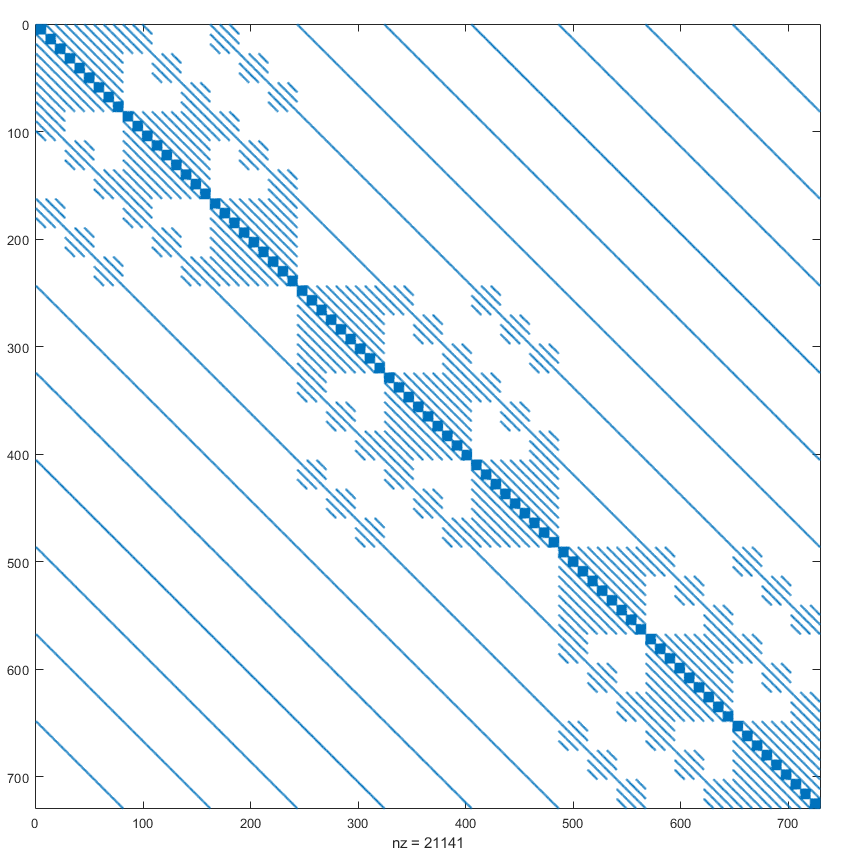
\includegraphics[width=0.5\linewidth]{spyQ.png}
    \caption{Sparsity pattern of the matrix \(U\)}
    \label{fig:Usparse}
\end{figure}

\noindent Then we can take the squares which have already been filled and turn them into constraints. So the constraint \(x_{i,j,k} = 1\) becomes 
\begin{align*}
    (x_{i,j,k} - 1)^2 &= x_{i,j,k}^2 - 2x_{i,j,k} + 1 \\
    &= -x_{i,j,k}^2 + 1
\end{align*}
which can be interpreted as subtracting 1 from the \((i,j,k)\)th element on the diagonal of \(U\). Doing this for every square which has been filled creates the matrix \(Q\).\\

\noindent Finally, solving the QUBO problem
\begin{align*}
    \min_{\mathbf{x} \in B(n)} \mathbf{x}^T Q \mathbf{x}
\end{align*}
will give us the \(\mathbf{x}\) which is a solution of the original Sudoku problem.\\

\noindent So the solution to the Sudoku is:

\hspace{92pt}\begin{lpsudoku}[scale=0.5]
\setrow{9}{\color{blue}6,\color{blue}5,8,2,4,\color{blue}7,\color{blue}9,1,\color{blue}3}
\setrow{8}{4,3,\color{blue}2,\color{blue}1,9,5,\color{blue}6,8,7}
\setrow{7}{\color{blue}9,1,7,8,\color{blue}6,\color{blue}3,2,5,\color{blue}4}
\setrow{6}{\color{blue}1,\color{blue}2,\color{blue}9,6,7,4,5,3,8}
\setrow{5}{\color{blue}3,7,\color{blue}4,\color{blue}9,6,\color{blue}8,\color{blue}1,6,2}
\setrow{4}{8,6,5,\color{blue}3,1,2,\color{blue}4,\color{blue}7,\color{blue}9}
\setrow{3}{2,9,\color{blue}6,7,\color{blue}8,1,\color{blue}3,4,\color{blue}5}
\setrow{2}{\color{blue}7,\color{blue}4,3,\color{blue}5,2,6,8,9,\color{blue}1}
\setrow{1}{\color{blue}5,\color{blue}8,\color{blue}1,\color{blue}4,3,9,7,\color{blue}2,\color{blue}6}
\end{lpsudoku}\\

\noindent The code for this QUBO implementation is on the GitHub under sudoku.m.\\
 
\noindent Unfortunately, since \(Q\) is so large it is often not feasible to use this implementation to obtain solutions to Sudoku problems. A more efficient implementation of Sudoku is derived in \cite{mücke2024sudoku}.\\

\noindent In this implementation the matrix \(Q\) is \(729 \times 729\). We could make this smaller by not including variables for squares which are filled. \\ 
Then assuming we are given \(17\) filled squares we can removing the variables representing these squares and so reduce the number of variables by \(17 \times 9 = 153\).\\
Since each filled square tells us the other squares on the same row, column or box have different values, \(24\) more variables are removed for each filled square. If we consider that \(\frac{17}{81}\) squares were already going to be removed, we can remove another \(\frac{64}{81} \times 24 \times 17 \approx 320\).\\

\noindent So we should be able to reduce the number of variables to \(\approx 260\) which should be more efficient. 

\section{Graph Isomorphism and Matching problems}
\subsection{The Graph Isomorphism problem}
Two graphs \(G_A\) and \(G_B\) are isomorphic if and only if there exists a bijection between the vertices of the graphs such that every edge which connects vertices in \(G_A\) corresponds to an edge connecting vertices in \(G_B\). \\
Essentially, an isomorphism means either graph can be redrawn and relabelled to be identical to the other. \\

\noindent So if the graphs have a different number of vertices or a different amount of edges, they cannot be isomorphic. You might think now that you can always find or rule out an isomorphism easily, but isomorphisms between graphs are not always obvious. For instance, can you tell if the graphs below are isomorphic?\\

\begin{figure}[H]
    \centering
    \hspace{48pt}
    \begin{subfigure}[h]{0.2\linewidth}
        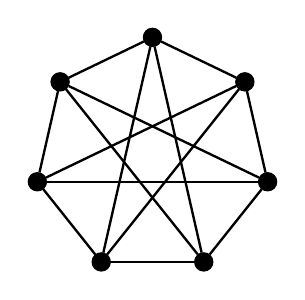
\begin{tikzpicture}
            \node[shape=circle,draw=black, fill=black, scale=0.7] (A) at (0, 1.5) {};
            \node[shape=circle,draw=black, fill=black, scale=0.7] (B) at (1.173, 0.935) {};
            \node[shape=circle,draw=black, fill=black, scale=0.7] (C) at (1.462, -0.334) {};
            \node[shape=circle,draw=black, fill=black, scale=0.7] (D) at (0.651, -1.352) {};
            \node[shape=circle,draw=black, fill=black, scale=0.7] (E) at (-0.651, -1.352) {};
            \node[shape=circle,draw=black, fill=black, scale=0.7] (F) at (-1.462, -0.334) {};
            \node[shape=circle,draw=black, fill=black, scale=0.7] (G) at (-1.173, 0.935) {};
        
            \path [line width=0.3mm] (A) edge node[left] {} (B);
            \path [line width=0.3mm] (A) edge node[left] {} (D);
            \path [line width=0.3mm] (A) edge node[left] {} (E);
            \path [line width=0.3mm] (A) edge node[left] {} (G);
        
            \path [line width=0.3mm] (B) edge node[left] {} (C);
            \path [line width=0.3mm] (B) edge node[left] {} (E);
            \path [line width=0.3mm] (B) edge node[left] {} (F);
        
            \path [line width=0.3mm] (C) edge node[left] {} (D);
            \path [line width=0.3mm] (C) edge node[left] {} (F);
            \path [line width=0.3mm] (C) edge node[left] {} (G);
        
            \path [line width=0.3mm] (D) edge node[left] {} (E);
            \path [line width=0.3mm] (D) edge node[left] {} (G);
        
            \path [line width=0.3mm] (E) edge node[left] {} (F);
        
            \path [line width=0.3mm] (F) edge node[left] {} (G);
        \end{tikzpicture}
    \end{subfigure}
    \hspace{40pt}
    \begin{subfigure}[h]{0.4\linewidth}
        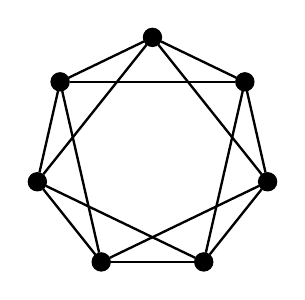
\begin{tikzpicture}
            \node[shape=circle,draw=black, fill=black, scale=0.7] (A) at (0, 1.5) {};
            \node[shape=circle,draw=black, fill=black, scale=0.7] (B) at (1.173, 0.935) {};
            \node[shape=circle,draw=black, fill=black, scale=0.7] (C) at (1.462, -0.334) {};
            \node[shape=circle,draw=black, fill=black, scale=0.7] (D) at (0.651, -1.352) {};
            \node[shape=circle,draw=black, fill=black, scale=0.7] (E) at (-0.651, -1.352) {};
            \node[shape=circle,draw=black, fill=black, scale=0.7] (F) at (-1.462, -0.334) {};
            \node[shape=circle,draw=black, fill=black, scale=0.7] (G) at (-1.173, 0.935) {};
        
            \path [line width=0.3mm] (A) edge node[left] {} (B);
            \path [line width=0.3mm] (A) edge node[left] {} (C);
        
            \path [line width=0.3mm] (B) edge node[left] {} (C);
            \path [line width=0.3mm] (B) edge node[left] {} (D);
        
            \path [line width=0.3mm] (C) edge node[left] {} (D);
            \path [line width=0.3mm] (C) edge node[left] {} (E);
        
            \path [line width=0.3mm] (D) edge node[left] {} (E);
            \path [line width=0.3mm] (D) edge node[left] {} (F);
        
            \path [line width=0.3mm] (E) edge node[left] {} (F);
            \path [line width=0.3mm] (E) edge node[left] {} (G);
        
            \path [line width=0.3mm] (F) edge node[left] {} (G);
            \path [line width=0.3mm] (F) edge node[left] {} (A);
        
            \path [line width=0.3mm] (G) edge node[left] {} (A);
            \path [line width=0.3mm] (G) edge node[left] {} (B);
        \end{tikzpicture}
    \end{subfigure}
    \caption{The graphs \(G_A\) (left) and \(G_B\) (right)}
    \label{fig:1}
\end{figure}

\noindent Now imagine trying to find an isomorphism between even larger graphs. Eventually, it is no longer possible to identify them by inspection and so we use algorithms to search for isomorphisms. \\

\noindent The graph isomorphism problem is the problem of determining whether any two graphs are isomorphic.\\

\noindent To interpret this as a QUBO problem we use some results from \autocite{klus2023continuous}. First,\\

\begin{lem}\label{lem:StochasticIso}
\cite[p.~6]{klus2023continuous} Suppose we have graphs \(G_A\) and \(G_B\) with adjacency matrices \(A\) and \(B\) respectively. The doubly stochastic relaxation of the graph isomorphism problem can be formulated as
\begin{equation*}
    c_D = \min_{X \in D(n)} ||XA - BX||^2_F,
\end{equation*}
where \(D(n)\) is the set of doubly stochastic matrices and \(||\cdot||_F\) denotes the Frobenius norm.
\end{lem}

\begin{lem}\label{lem:qubo1}
    \cite[p.~8]{klus2023continuous} This optimisation problem can be written as \begin{align*}
    \min_{\substack{\mathbf{x} \in B(n) \\ C\mathbf{x} = d}} \mathbf{x}^T H\mathbf{x},
    \end{align*}
    where \(\mathbf{x} = \text{vec}(X)\), \(H = (A \otimes I_n - I_n \otimes B)^2\), and \(C\), \(d\) are defined by (\ref{mat:CD}).
\end{lem}

\noindent Since we have shown in (\ref{penalty:CX}) that the constraint \(C\mathbf{x} = d\) corresponds to the penalty \(\mathbf{x}^T(C^T C - 2\text{diag}(C^T d))\mathbf{x}\), a QUBO formulation of this problem can be written as 
\begin{equation}\label{QUBO: graphIso1}
	\min_{x \in B(n)} \mathbf{x}^T Q \mathbf{x},
\end{equation}
where \(Q = H + \lambda C^T C - 2\lambda\text{diag}(C^T d)\) and \(\lambda\) is the penalty weight.\\

\noindent Alternatively, we can use Lemma 4.15 which states
\begin{lem}
	\cite[p.~13]{klus2023continuous} The optimisation problem can be written as \begin{align*}
		\min_{\substack{\mathbf{x} \in B(n) \\ C\mathbf{x} = d \\ H\mathbf{x}=0}} -\mathbf{x}^T\mathbf{x},
	\end{align*}
	where \(\mathbf{x}, C, d\) and \(H\) are defined as in (\ref{lem:qubo1})
\end{lem}

\noindent Since the constraint \(H\mathbf{x} = 0\) corresponds to the penalty \(H\mathbf{x} \cdot H\mathbf{x} =  \mathbf{x}^T H^T H  \mathbf{x}\) we can write a QUBO formulation of this problem as

\begin{equation}\label{QUBO: graphIso2}
	\min_{x \geq 0} \mathbf{x}^T Q \mathbf{x}
\end{equation}
where \(Q = -I_n + \lambda_1 C^T C - 2\lambda_1\text{diag}(C^T d) + \lambda_2 H^T H\) with penalty weights \(\lambda_1\) and \(\lambda_2\).\\

\noindent When we compare both QUBO implementations for the problem we find that generally implementation (\ref{QUBO: graphIso1}) is faster.

\subsubsection{Example: Graph Isomorphism problem}
Consider the graphs \(G_A\) and \(G_B\) from Figure \ref{fig:1}. \\

\noindent These graphs have the adjacency matrices
\begin{align*}
    A = \begin{pmatrix}
        0 & 1 & 0 & 1 & 1 & 0 & 1 \\
        1 & 0 & 1 & 0 & 1 & 1 & 0 \\
        0 & 1 & 0 & 1 & 0 & 1 & 1 \\
        1 & 0 & 1 & 0 & 1 & 0 & 1 \\
        1 & 1 & 0 & 1 & 0 & 1 & 0 \\
        0 & 1 & 1 & 0 & 1 & 0 & 1 \\
        1 & 0 & 1 & 1 & 0 & 1 & 0
    \end{pmatrix} \: \text{and }
    B = \begin{pmatrix}
        0 & 1 & 1 & 0 & 0 & 1 & 1 \\
        1 & 0 & 1 & 1 & 0 & 0 & 1 \\
        1 & 1 & 0 & 1 & 1 & 0 & 0 \\
        0 & 1 & 1 & 0 & 1 & 1 & 0 \\
        0 & 0 & 1 & 1 & 0 & 1 & 1 \\
        1 & 0 & 0 & 1 & 1 & 0 & 1 \\
        1 & 1 & 0 & 0 & 1 & 1 & 0
    \end{pmatrix},
\end{align*}
when we enumerate their vertices clockwise. If we substitute \(A, B\) into (\ref{QUBO: graphIso1}), choose \(\lambda = 10\), and solve the QUBO problem we get
\begin{align*}
    X = \begin{pmatrix}
        0 & 1 & 0 & 0 & 0 & 0 & 0 \\
        0 & 0 & 0 & 0 & 0 & 1 & 0 \\
        0 & 0 & 1 & 0 & 0 & 0 & 0 \\
        0 & 0 & 0 & 0 & 0 & 0 & 1 \\
        0 & 0 & 0 & 1 & 0 & 0 & 0 \\
        1 & 0 & 0 & 0 & 0 & 0 & 0 \\
        0 & 0 & 0 & 0 & 1 & 0 & 0
    \end{pmatrix}
\end{align*}
which we find represents an isomorphism between \(G_A\) and \(G_B\).\\

\noindent Using this we find that the labelling  
\begin{figure}[H]
    \centering
    \hspace{48pt}
    \begin{subfigure}[h]{0.2\linewidth}
        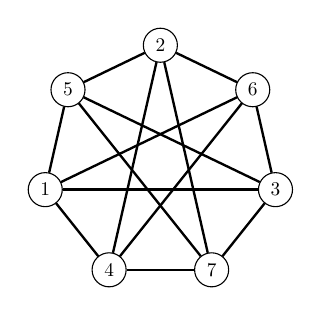
\begin{tikzpicture}
            \node[shape=circle,draw=black, scale=0.7] (A) at (0, 1.5) {2};
            \node[shape=circle,draw=black, scale=0.7] (B) at (1.173, 0.935) {6};
            \node[shape=circle,draw=black, scale=0.7] (C) at (1.462, -0.334) {3};
            \node[shape=circle,draw=black, scale=0.7] (D) at (0.651, -1.352) {7};
            \node[shape=circle,draw=black, scale=0.7] (E) at (-0.651, -1.352) {4};
            \node[shape=circle,draw=black, scale=0.7] (F) at (-1.462, -0.334) {1};
            \node[shape=circle,draw=black, scale=0.7] (G) at (-1.173, 0.935) {5};
        
            \path [line width=0.3mm] (A) edge node[left] {} (B);
            \path [line width=0.3mm] (A) edge node[left] {} (D);
            \path [line width=0.3mm] (A) edge node[left] {} (E);
            \path [line width=0.3mm] (A) edge node[left] {} (G);
        
            \path [line width=0.3mm] (B) edge node[left] {} (C);
            \path [line width=0.3mm] (B) edge node[left] {} (E);
            \path [line width=0.3mm] (B) edge node[left] {} (F);
        
            \path [line width=0.3mm] (C) edge node[left] {} (D);
            \path [line width=0.3mm] (C) edge node[left] {} (F);
            \path [line width=0.3mm] (C) edge node[left] {} (G);
        
            \path [line width=0.3mm] (D) edge node[left] {} (E);
            \path [line width=0.3mm] (D) edge node[left] {} (G);
        
            \path [line width=0.3mm] (E) edge node[left] {} (F);
        
            \path [line width=0.3mm] (F) edge node[left] {} (G);
        \end{tikzpicture}
    \end{subfigure}
    \hspace{40pt}
    \begin{subfigure}[h]{0.4\linewidth}
        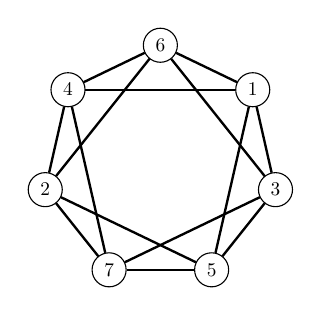
\begin{tikzpicture}
            \node[shape=circle,draw=black, scale=0.7] (A) at (0, 1.5) {6};
            \node[shape=circle,draw=black, scale=0.7] (B) at (1.173, 0.935) {1};
            \node[shape=circle,draw=black, scale=0.7] (C) at (1.462, -0.334) {3};
            \node[shape=circle,draw=black, scale=0.7] (D) at (0.651, -1.352) {5};
            \node[shape=circle,draw=black, scale=0.7] (E) at (-0.651, -1.352) {7};
            \node[shape=circle,draw=black, scale=0.7] (F) at (-1.462, -0.334) {2};
            \node[shape=circle,draw=black, scale=0.7] (G) at (-1.173, 0.935) {4};
    
            \path [line width=0.3mm] (A) edge node[left] {} (B);
            \path [line width=0.3mm] (A) edge node[left] {} (C);
        
            \path [line width=0.3mm] (B) edge node[left] {} (C);
            \path [line width=0.3mm] (B) edge node[left] {} (D);
        
            \path [line width=0.3mm] (C) edge node[left] {} (D);
            \path [line width=0.3mm] (C) edge node[left] {} (E);
        
            \path [line width=0.3mm] (D) edge node[left] {} (E);
            \path [line width=0.3mm] (D) edge node[left] {} (F);
        
            \path [line width=0.3mm] (E) edge node[left] {} (F);
            \path [line width=0.3mm] (E) edge node[left] {} (G);
        
            \path [line width=0.3mm] (F) edge node[left] {} (G);
            \path [line width=0.3mm] (F) edge node[left] {} (A);
        
            \path [line width=0.3mm] (G) edge node[left] {} (A);
            \path [line width=0.3mm] (G) edge node[left] {} (B);
        \end{tikzpicture}
    \end{subfigure}
\end{figure}
\noindent is an isomorphism.\\

\noindent The code for this implementation is
\begin{lstlisting}[language=MATLAB]
H = (kron(A, eye(n)) - kron(eye(n), B))^2;
Q = H + weight*(Ct*C - 2*diag(Ct*d));

x = solve(qubo(Q));
mat = reshape(x.BestX, [n,n]);
\end{lstlisting}

\subsection{Graph Matching and Quadratic Assignment problem}

\subsubsection{Graph Matching}

Given two weighted graphs \(G_A\) and \(G_B\), the graph matching problem is the problem of finding the bijection between the vertices of \(G_A\) and \(G_B\) which minimises the edge difference.\\

\noindent Essentially, the graph matching problem is a generalisation of the graph isomorphism problem but instead of determining if the graphs are isomorphic we want to find the closest bijection between the graphs.
The graph matching problem can be formulated as (\ref{lem:StochasticIso}) where \(A,B\) are weighted adjacency matrices. This means that it is equivalent to (\ref{lem:qubo1}) following the steps in \cite{klus2023continuous}.\\

\noindent So, the QUBO formulation of the graph matching problem is
\begin{equation*}
	\min_{\mathbf{x} \in B(n)} \mathbf{x}^T Q \mathbf{x}
\end{equation*}
where \(Q = (A \otimes I_n - I_n \otimes B)^2 + \lambda C^T C - 2\lambda\text{diag}(C^T d)\), \(\lambda\) is the penalty weight and \(C\), \(d\) are defined by \ref{mat:CD}.\\

\subsubsection{Example: Graph Matching}

Consider the graphs \(G_L\) and \(G_R\) on the left and right respectively. 
\begin{figure}[H]
    \centering
    \hspace{48pt}
    \begin{subfigure}[h]{0.2\linewidth}
        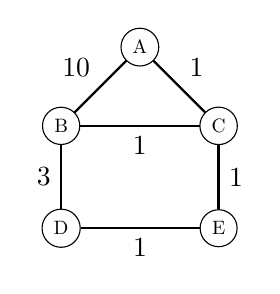
\begin{tikzpicture}
            \node[shape=circle,draw=black, scale=0.7] (A) at (0, 0) {A};
            \node[shape=circle,draw=black, scale=0.7] (B) at (-1, -1) {B};
            \node[shape=circle,draw=black, scale=0.7] (C) at (1, -1) {C};
            \node[shape=circle,draw=black, scale=0.7] (D) at (-1, -2.3) {D};
            \node[shape=circle,draw=black, scale=0.7] (E) at (1, -2.3) {E};
        
            \path[line width=0.3mm] (A) edge node[above left]{10} (B);
            \path [line width=0.3mm] (A) edge node[above right]{1} (C);

            \path [line width=0.3mm] (B) edge node[below]{1} (C);
            \path [line width=0.3mm] (B) edge node[left]{3} (D);

            \path [line width=0.3mm] (E) edge node[right]{1} (C);
            \path [line width=0.3mm] (E) edge node[below]{1} (D);
            
        \end{tikzpicture}
    \end{subfigure}
    \hspace{40pt}
    \begin{subfigure}[h]{0.4\linewidth}
        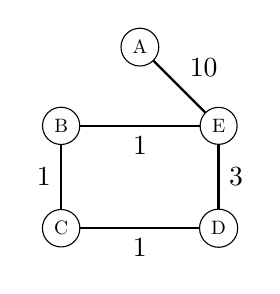
\begin{tikzpicture}
            \node[shape=circle,draw=black, scale=0.7] (A) at (0, 0) {A};
            \node[shape=circle,draw=black, scale=0.7] (B) at (-1, -1) {B};
            \node[shape=circle,draw=black, scale=0.7] (E) at (1, -1) {E};
            \node[shape=circle,draw=black, scale=0.7] (C) at (-1, -2.3) {C};
            \node[shape=circle,draw=black, scale=0.7] (D) at (1, -2.3) {D};
        
            \path[line width=0.3mm] (A) edge node[above right]{10} (E);

            \path[line width=0.3mm] (E) edge node[below]{1} (B);
            \path[line width=0.3mm] (E) edge node[right]{3} (D);

            \path[line width=0.3mm] (C) edge node[left]{1} (B);
            \path[line width=0.3mm] (C) edge node[below]{1} (D);
            
        \end{tikzpicture}
    \end{subfigure}
\end{figure}
\noindent These graphs have the adjacency matrices
\begin{align*}
    L = \begin{pmatrix}
        0 & 10 & 1 & 0 & 0 \\
        10 & 0 & 1 & 3 & 0 \\
        1 & 1 & 0 & 0 & 1 \\
        0 & 3 & 0 & 0 & 1 \\
        0 & 0 & 1 & 1 & 0
    \end{pmatrix}, \quad R = \begin{pmatrix}
        0 & 0 & 0 & 0 & 10 \\
        0 & 0 & 1 & 0 & 1 \\
        0 & 1 & 0 & 1 & 0 \\
        0 & 0 & 1 & 0 & 3 \\
        10 & 1 & 0 & 3 & 0
    \end{pmatrix}.
\end{align*}

\noindent Using these matrices, we find the solution of the graph matching problem is the permutation matrix
\begin{align*}
    X = \begin{pmatrix}
        1 & 0 & 0 & 0 & 0 \\
        0 & 0 & 1 & 0 & 0 \\
        0 & 0 & 0 & 0 & 1 \\
        0 & 0 & 0 & 1 & 0 \\
        0 & 1 & 0 & 0 & 0
    \end{pmatrix}
\end{align*}
which corresponds to the mapping from \(G_L\) to \(G_R\) which takes \(A \mapsto A, B \mapsto E, C \mapsto B, D \mapsto D\) and \(E \mapsto C\).

\subsubsection{Quadratic Assignment}

The quadratic assignment problem can be stated as:

Suppose we are given a set of \(n\) facilities and \(n\) locations, our job is to allocate each facility to a location such that we minimise the total cost. Each pair of facilities has a required flow and each pair of locations has a distance. The cost function is the sum of the flows multiplied by the distance for each facility-location pair.\\

\noindent Many real-world problems such to optimising building layouts, hospital transportation and scheduling can be expressed as quadratic assignment problems.\\

\noindent We can obtain a QUBO formulation of this as follows: \\
First let \(F\) and \(D\) be the flow and distance matrices where entries \(F_{ij}\) are the required flow between facilities \(i\) and \(j\) and \(D_{ij}\) is the distance between locations \(l_i\) and \(l_j\). Then the problem can be expressed as:
\begin{align*}
    \min_{X \in \mathcal{P}(n)} \: \text{tr}(FXD^TX^T).
\end{align*}

\noindent Using \cite[p.~3]{klus2023continuous} since \(X\) is a permutation matrix we have
\begin{align*}
    2\text{tr}(FXD^TX^T) = ||F||_F^2 + ||D||_F^2 - ||XF - DX||_F^2.
\end{align*}

\noindent Therefore minimising \(\text{tr}(FXD^TX^T)\) is equivalent to maximising \(||XF - DX||_F^2\) which is the negation of (\ref{lem:StochasticIso}) so the QUBO formulation of the quadratic assignment problem is the negation of (\ref{lem:qubo1})
\begin{equation*}
	\min_{\mathbf{x} \in B(n)} \mathbf{x}^T Q \mathbf{x}
\end{equation*}
where \(Q = -(A \otimes I_n - I_n \otimes B)^2 + \lambda C^T C -\lambda\text{diag}(C^T d)\), \(\lambda\) is the penalty weight and \(C\), \(d\) are defined by \ref{mat:CD}.\\

\section{Quantum Annealing}

One of the main reasons for constructing QUBO formulations of problems is that they are well-suited to being solved using quantum annealing. In this section we detail the connection between QUBO problems and quantum annealers. 

\subsection{Ising models}

First we need to modify our QUBO problems slightly to obtain the Ising models which quantum annealers are designed to solve.
Recall that the general form of a QUBO problem is
\begin{align*}
    \min_{x \in B(n)} \: f(\mathbf{x}) = \mathbf{x}^T Q \mathbf{x} + d.
\end{align*}

\noindent An Ising problem is an optimisation problem where the objective function is a quadratic function of multiple variables and each variable is either -1 or 1 (which are referred to as spins). We can convert a QUBO problem to an Ising formulation by applying the linear mapping \(s_i = 2x_i - 1\). The objective function values will then differ by 
\begin{align*}
    \mathbf{x}^T Q \mathbf{x} + d = \frac{1}{4} (\mathbf{s}^T + J_{1,n})Q(\mathbf{s} + J_{n,1}) + d 
\end{align*} 
where \(J_{i,j}\) is the \(i \times j\) matrix of ones.\\

\noindent The objective function of the Ising formulation is referred to as the energy (so that the optimal solution corresponds to the lowest energy). 

\subsection{Quantum Annealers}

\noindent This section is an abridged explanation of some of the ideas behind quantum annealing. For a more detailed explanation see \cite{tasseff2022emergingpotentialquantumannealing} and \cite{Yarkoni_2022}.\\

\noindent The idea behind quantum annealing is as follows. First we create an Ising formulation of the target problem, and label the objective we are looking to minimise the final Hamiltonian.

\noindent Then we prepare a quantum system in its ground state of an easy to solve function known as the initial Hamiltonian. If we slowly interpolate between the initial and the final Hamiltonian, the Adiabatic theorem \cite{Yarkoni_2022} ensures that the quantum system remains in the ground state. At the end, this ground state will correspond to the optimal solution of the target problem.\\

\noindent This process is analogous the the technique of annealing metal where a metal is heated above its recrystallization temperature and slowly cooled to increase strength and reduce stress.

\noindent A great explanation of the physical mechanism underlying quantum annealing is given in \cite{quantumAnnealingDWave} by D-Wave Systems who are the leading providers of quantum annealers. \\

\subsection{Limitations}
\label{sec:limitations}

As shown in \cite{tasseff2022emergingpotentialquantumannealing}, there is some evidence that quantum annealers can provide a performance advantage for certain problems. But this advantage has not been conclusively demonstrated over the fastest classical algorithms.\\

\noindent The largest commercial quantum annealer is D-Wave System's 5000 qubit Advantage system \cite{DWaveSystemsAdvantage}. This system allows each 15 couplers per qubit effectively means each column in the QUBO matrix must have less than 16 entries. This could mean that some QUBO formulations are infeasible to solve using the Advantage system.\\

\noindent Unfortunately the MATLAB code provided is not yet compatible with D-Wave Systems quantum annealers. But it should all be compatible with IBM's remote Qiskit service. 

\section{Conclusion}

In this project we showed how many combinatorial optimization problems can be naturally expressed as QUBO problems (with particular attention to the graph isomorphism problem). As research into QUBO problems and quantum annealers continues, we will hopefully develop formulations for more problems and overcome the limitations in \ref{sec:limitations}.  

\subsection{Acknowledgements}

\noindent Thank you to my supervisor Dr Stefan Klus for his guidance and help throughout this project.\\

\noindent This project was funded by the Edinburgh Mathematical Society. 

\newpage

\nocite{*}
\printbibliography % This command prints the cited references.

\end{document}
